\documentclass[runningheads]{llncs}

\usepackage[backend=biber]{biblatex}
\bibliography{../../AGI-book}

\usepackage[T1]{fontenc}
% T1 fonts will be used to generate the final print and online PDFs,
% so please use T1 fonts in your manuscript whenever possible.
% Other font encondings may result in incorrect characters.
%
\usepackage{graphicx}
% Used for displaying a sample figure. If possible, figure files should
% be included in EPS format.
%
% If you use the hyperref package, please uncomment the following two lines
% to display URLs in blue roman font according to Springer's eBook style:
%\usepackage{color}
%\renewcommand\UrlFont{\color{blue}\rmfamily}

\usepackage{amsmath}
\usepackage{amssymb}    % for \rightsquigarrow
\usepackage{wasysym}	% for frown face
\usepackage{mathrsfs} 	% for \mathscr
\usepackage{stmaryrd}
\usepackage{mathtools}		% to extend length of double harpoon arrows

\begin{document}
%
\title{AGI from the perspectives of Categorical Logic and Algebraic Geometry}
%
%\titlerunning{Abbreviated paper title}
% If the paper title is too long for the running head, you can set
% an abbreviated paper title here
%
\author{King-Yin Yan \orcidID{0009-0007-8238-2442}}
%
\authorrunning{K-Y. Yan}
% First names are abbreviated in the running head.
% If there are more than two authors, 'et al.' is used.
%
\institute{\email{general.intelligence@gmail.com}}
%
\maketitle              % typeset the header of the contribution
%
\begin{abstract}
To ``situate'' AGI in the context of some current mathematics, so that readers can more easily see whether current mathematical ideas can be fruitfully applied to AGI.

\keywords{AGI  \and categorical logic \and Curry-Howard isomorphism \and homotopy type theory  \and algebraic geometry \and topos theory.}
\end{abstract}
%
%
%
\section{Goal of this paper}

The bottleneck of AGI development is the speed of learning algorithms.  The daily cost of training GPT-4 was rumored to be \$100M by Sam Altman.  To speed up learning, one needs \textbf{inductive biases}, according to the \textbf{No Free Lunch theorem} \cite{Wolpert1997} \cite{Wikipedia-no-free-lunch}.  A principled way to introduce inductive bias is by the structure of logic.  The reason being that, if humans have discovered the structure of logic in this world, an intelligent program may re-discover the same structure.  So our question is:  what is the mathematical structure of logic?

% Traditionally this line of research is called algebraic logic, starting from Leibniz and Boole, up to more recent times Tarski's cylindrical algebra and Paul Halmos' work.  

\section{Conclusions thus far}

The conclusions of this paper are mostly \textit{negative}.  That is to say, the mathematical structures described here seem unable to offer practical ways to accelerate AGI, unless the reader can discover more ingenious ideas.  Nevertheless the author hopes the presentation of these ideas thus far can help the readers on their way.

In each section below, we look at one aspect of the categorical structure of logic and speculate on how it might aid AGI architecture.

\subsection{Where is GPT?}

\begin{figure}
	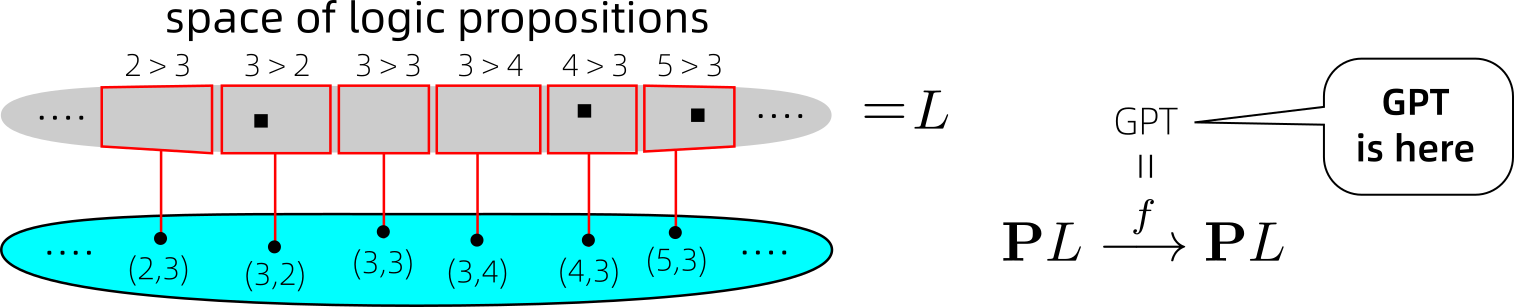
\includegraphics[scale=.5]{GPT-is-here.png}
	\caption{(Left) A sheaf of propositions over pairs of natural numbers; (Right) The function space where GPT lives.}
	\label{fig:GPT-is-here}
\end{figure}

GPT \cite{chatGPT2020} can be regarded as a \textbf{logic consequence operator} mapping from the space of propositions to itself (as a \textbf{set-valued map}), as shown in Fig.\ref{fig:GPT-is-here}.

\begin{figure}
	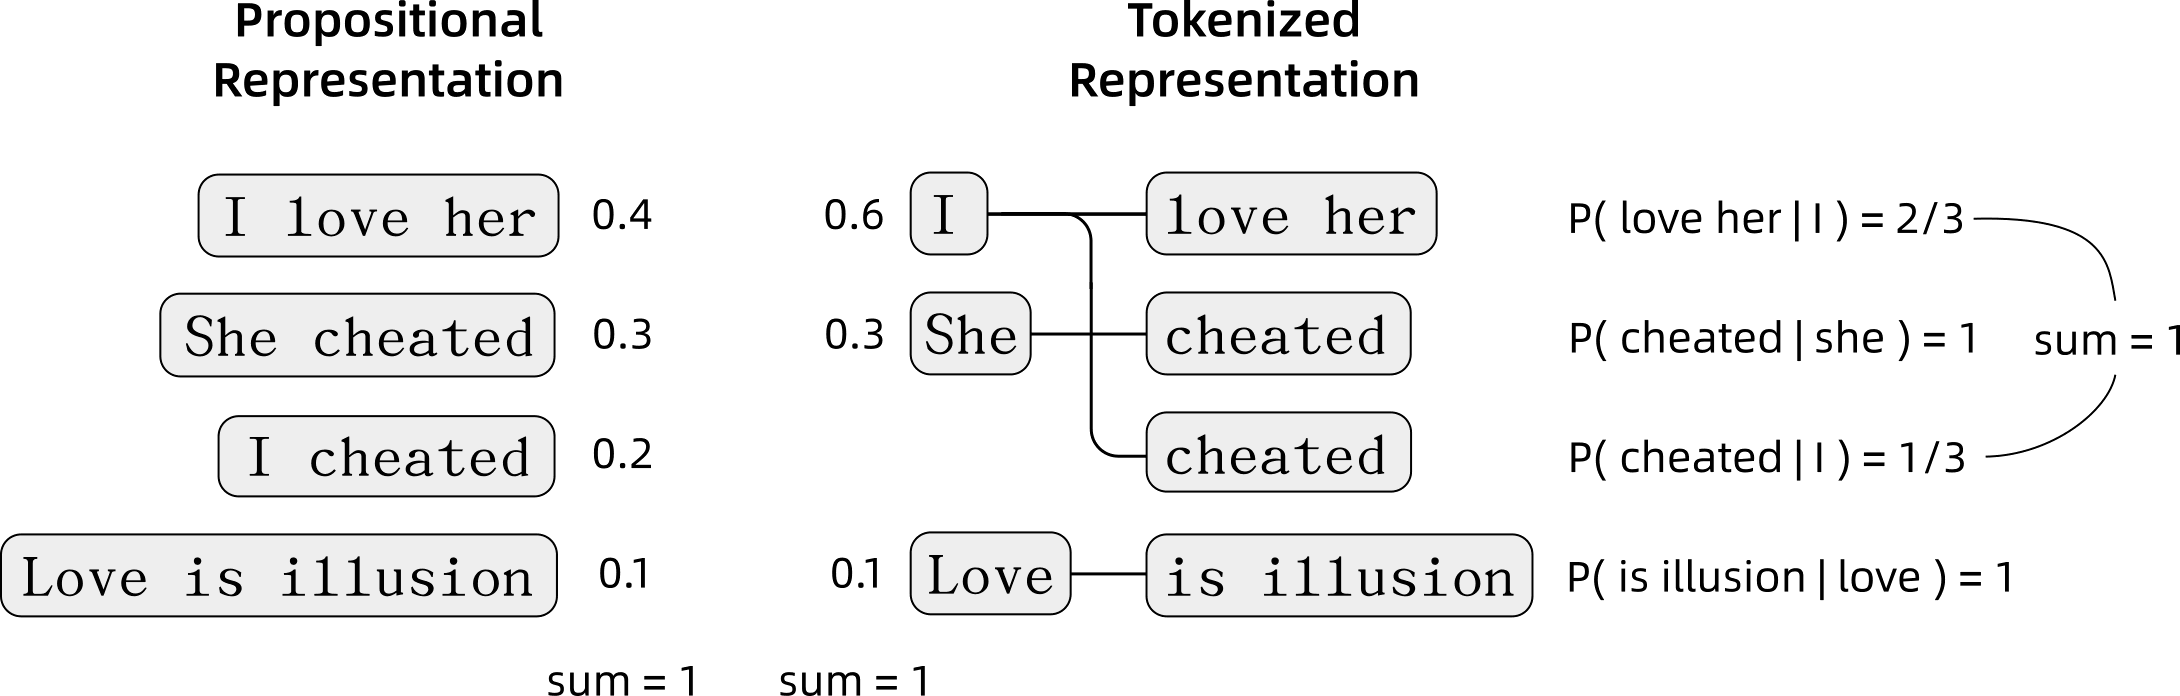
\includegraphics[scale=.4]{I-love-her-she-is-bitch.png}	% width=\textwidth
	\caption{The equivalence of probability distributions over propositions and over tokens. For simplicity the decomposition for just the leading token is shown.} \label{fig:she-is-bitch}
\end{figure}

Without loss of generality, GPT can be seen as acting on propositions, as probability distributions on tokens are equivalent to probability distributions on sentences (propositions), see Fig. \ref{fig:she-is-bitch}.

To what extent can we say that GPT outputs a vector in a Curry-Howard type-theoretic space?  A neural network (eg. GPT) always maps an input to the the same output vector, as it is a \textit{deterministic} map. Thus it seems meaningless to ask what is the meaning of the \textit{neighborhood} of an output vector, if the network never goes there during inference time.

\begin{figure}
	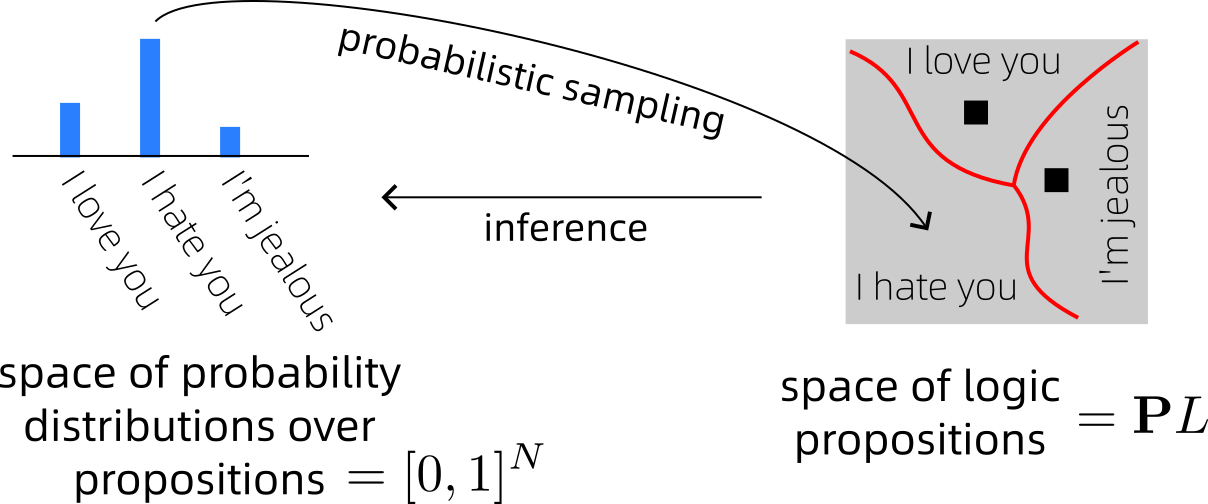
\includegraphics[scale=.4]{Transformer-output.png} \qquad
	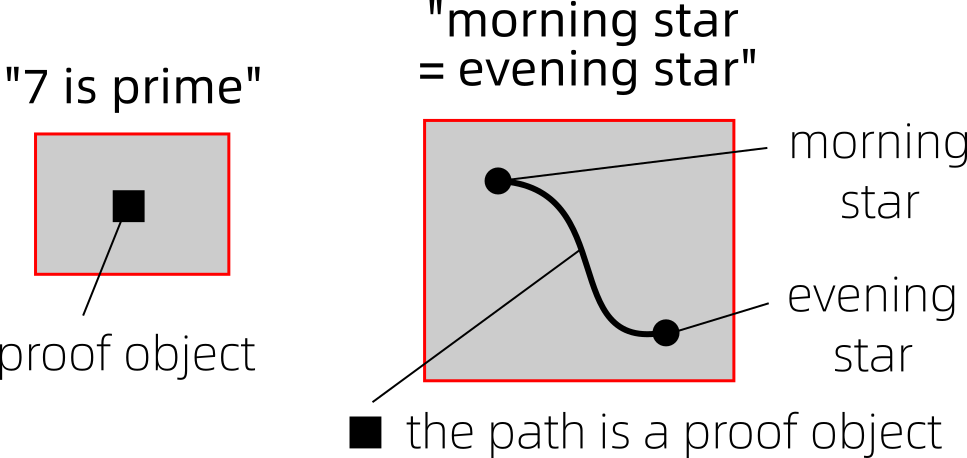
\includegraphics[scale=.35]{morning-star.png}
	\caption{(Left) How probabilistic inference in GPT results in deterministic vector positions; (Right) In HoTT, a path is a proof object of an identity type.}
	\label{fig:morning-star}
\end{figure}

Fig.\ref{fig:morning-star}(Left) illustrates why even despite probabilistic sampling, the outputs of GPT seem to follow fixed trajectories (as soon as learning has finished).  Nevertheless, if we artificially ``perturb'' the input, the output probability distribution will change \textit{smoothly}, say from favoring token $A$ to favoring token $B$, as neural networks are always \textit{differentiable} functions.  One can define the \textbf{boundary} between tokens $A$ and $B$ as where their probabilities reverse in magnitude.  This forms a Voronoi-like tessellation of the output space that can be regarded as Curry-Howard type-spaces.

\subsection{Homotopy type theory}

For a neural network to process HoTT information, it needs a way to 

Therefore we can conclude that current neural networks are unlikely to process HoTT structures.

\subsection{Commutativity of $\wedge$ and $\vee$}

Permutation symmetry is the easiest to recognize and implement \cite{Zaheer2017} \cite{Qi2017}.  It is well-known the Transformer is \textbf{equivariant} to permutations of inputs.  This may be seen as evidence that Transformer \textbf{tokens} are proposition-like entities, with the caveat that we may be confusing the propositional level with the sub-propositional level of atomic concepts.  An easy-to-remember example is: $I \heartsuit U \neq U \heartsuit I$, but $I \heartsuit U \wedge U \heartsuit I = U \heartsuit I \wedge I \heartsuit U$.

\subsection{$\forall$ and $\exists$ as adjunctions}

It seems difficult to translate this structure into a structural modification of neural networks.  From our experience in logic-based AI, logic rules are usually implicitly $\forall$-quantified, and $\exists$ is usually implicit by the \textbf{Closed-World Assumption}.

The following two conditions concern the well-behavior of quantification, as described in \cite{Jacobs1999} and on nLab \cite{nLab-beck-chevalley} \cite{nLab-Frobenius}:

\noindent The \textbf{Beck-Chevalley condition} says that substitution of free variables commutes with quantification.

\noindent The \textbf{Frobenius condition} corresponds in logic to saying that $\exists x. (\phi \wedge \psi)$ is equivalent to $(\exists x. \phi) \wedge \psi$ if $x$ is not free in $\psi$.

Both conditions are ``self-evident'' from the logic perspective, but it remains to be seen how they can be applied to neural networks.

\subsection{Predicates as fibration}

The relevant mental picture here is Fig.\ref{fig:GPT-is-here}(Left). 

\subsection{Iteration of $\vdash$ and Looped Transformers}

\subsection{Modal logic}

Grothendieck topology is re-captured as a modal operator.

\begin{figure}
	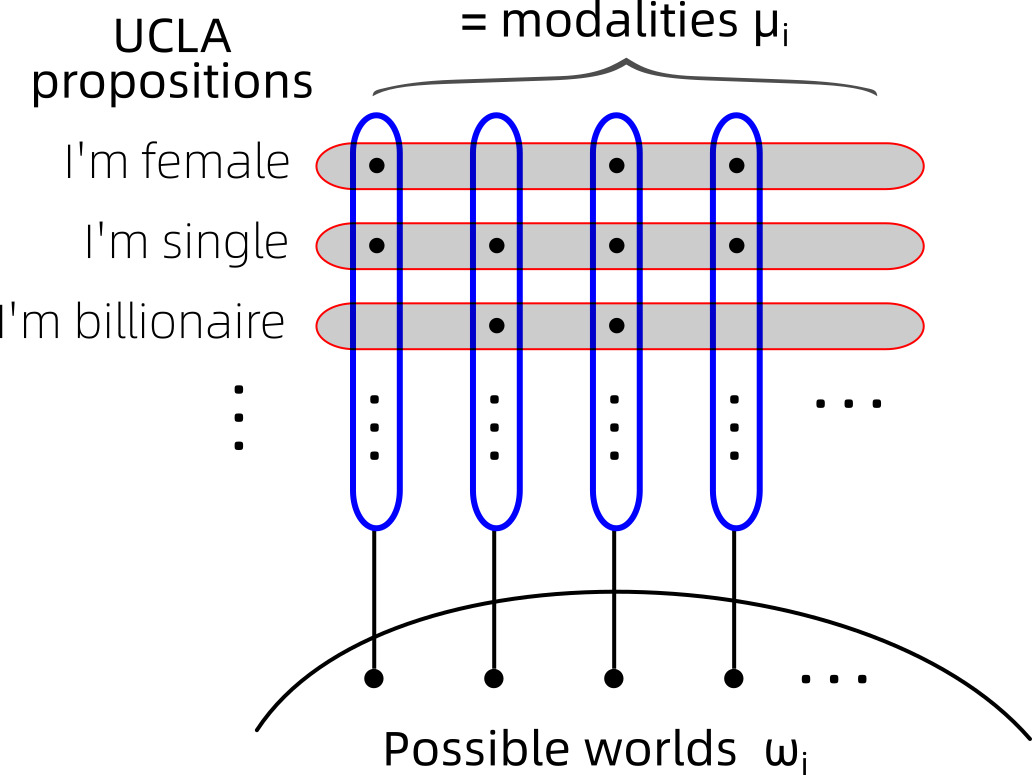
\includegraphics[scale=.4]{possible-worlds-as-sheaf.png} \qquad
	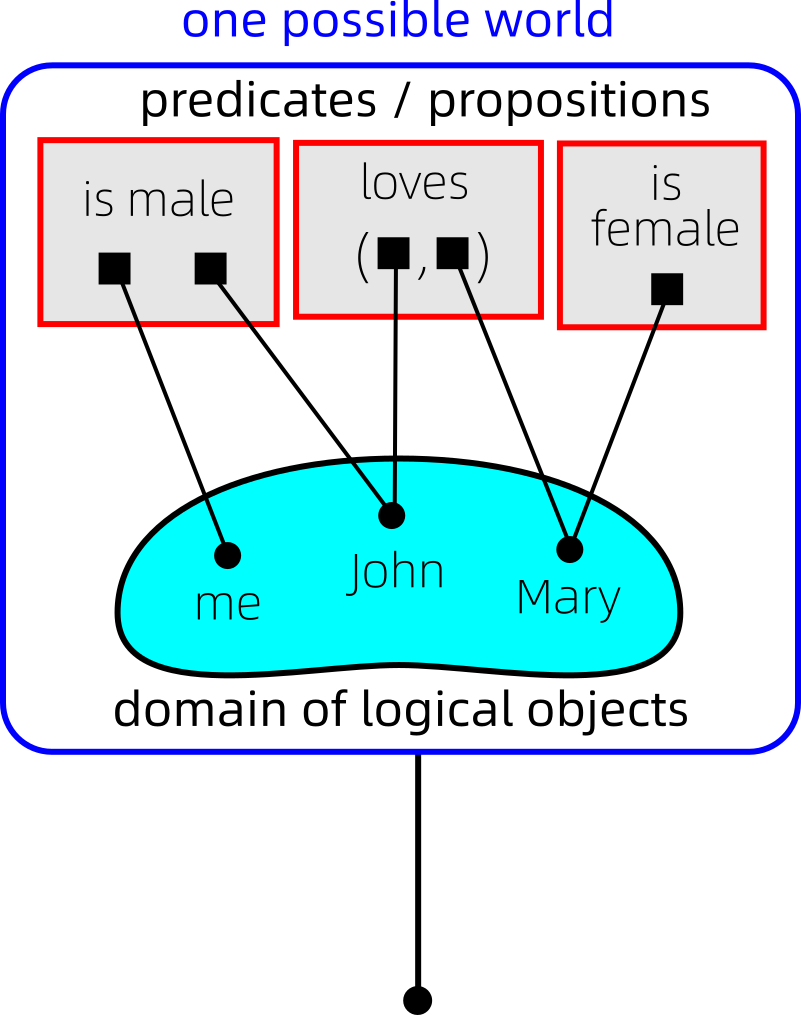
\includegraphics[scale=.35]{possible-world-single-example.png}
	\caption{(Left) The set underneath are indexes to possible worlds, for example $\omega_i = \{1,2,3...\}$. Each ``stalk'' represents a possible world, together they form a fibration over the base space.}
	\label{fig:possible-worlds-as-sheaf}
\end{figure}

\subsection{Algebraic geometry}

The fundamental duality in algebraic geometry is:
\begin{equation}
\left\{ \begin{tabular}{cc} spaces, or \\ varieties \end{tabular} \right\} \longleftrightarrow \left\{ \begin{tabular}{cc} commutative \\ $\mathbf{k}$-algebras \end{tabular} \right\}
\end{equation}
within this correspondence, ``points'' in geometry are identified with \textbf{prime ideals}.
%\begin{equation}
%\left\{ \begin{tabular}{cc} points in \\ geometry \end{tabular} \right\} \longleftrightarrow \left\{ \begin{tabular}{cc} prime ideals \end{tabular} \right\}
%\end{equation}

An approach suggested by Yuri Manin is to turn logic into an algebra, such as the Boolean ring (but this can only handle propositional logic).  Varieties defined by such Boolean polynomials \cite{Lundqvist2015} live in the space $\mathbb{Z}_2^n$, the \textbf{discrete hypercube}.  

My visualization of the ``Grothendieck picture'' of AGI is like this:
\begin{equation}
\vcenter{\hbox{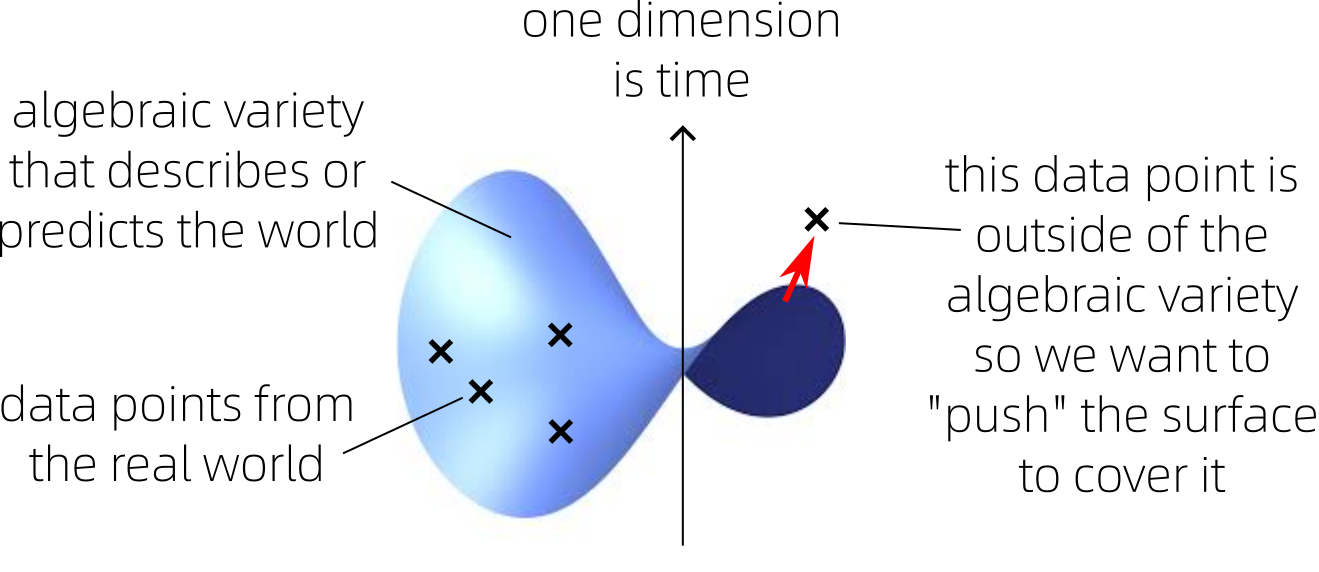
\includegraphics[scale=0.4]{Grothendieck-picture.png}}} \nonumber
\end{equation}

One of the interesting discoveries in categorical logic is that every topos admits an \textbf{internal language}.  This is a simple consequence of Curry-Howard: since a type-space corresponds to a logic proposition, and categorical logic interprets type-spaces as objects in a category, thus every category (satisfying extra conditions) can be interpreted as having an ``internal'' logic.  The converse of this correspondence is the \textbf{classifying topos} of a logic theory $\mathbb{T}$:
\begin{equation}
\underset{\footnotesize\text{classifying topos}}{\mathcal{E}_\mathbb{T}} \xrightleftharpoons[]{\; \text{ internal language } \;} \underset{\footnotesize\text{theory}}{\mathbb{T}}
\end{equation}

Olivia Caramello \cite{Caramello2018} developed an idea where toposes play the central role of ``bridges'' that transfer information between theories (AGI can be seen as the \textbf{common-sense theory} of our physical world).  She showed that for any geometric theory $\mathbb{T}$, interpreted in the Grothendieck topos $\mathcal{E}_\mathbb{T}$, there is a \textbf{universal} model $U$ such that any model of $\mathbb{T}$ up to isomorphism is a pullback of $U$ along a geometric morphism.  This means that the \textbf{classifying topos} of $\mathbb{T}$ is the \textbf{representing object} in a \textbf{Yoneda lemma}\footnote{The Yoneda lemma can be understood as saying some object in a category is able to ``represent'' the entire category.  A archetypal example is \textbf{Cayley's theorem} in group theory, that says that every finite group is isomorphic to a subgroup of the symmetric group $\mathfrak{S}_n$. Here the symmetric group is the \textbf{representing object} capable of representing all finite groups.}.  A diagram in her book is reproduced here with simplifications in Fig.\ref{fig:Caramello-pic}(Left).

\begin{figure}
	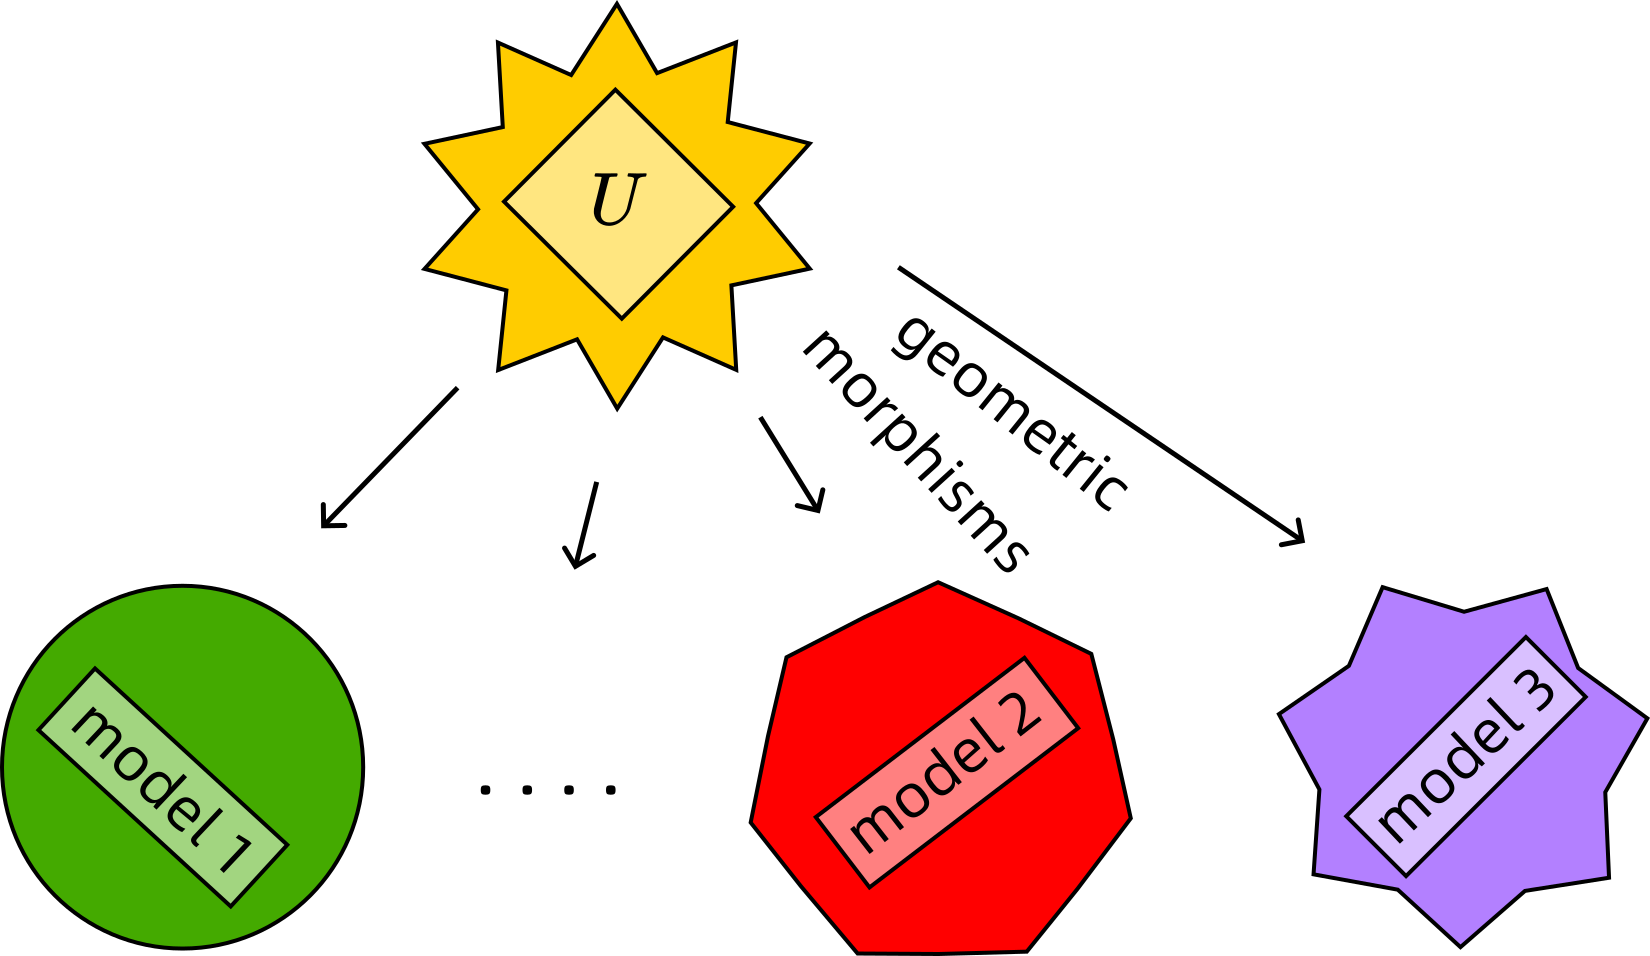
\includegraphics[scale=.25]{Caramello-picture.png} \qquad
	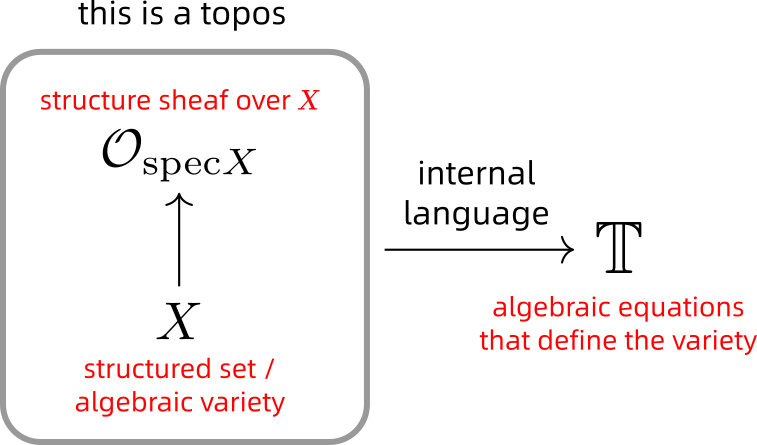
\includegraphics[scale=.5]{geometric-topos.png}
	\caption{(Left) The universal model $U$ inside its classifying topos (darker color); (Right) The classical formulation of algebraic geometry}
	\label{fig:Caramello-pic}
\end{figure}

In a similar vein, Ingo Blechschmidt's PhD thesis \cite{Blechschmidt2017} and his IHES presentation 9 years ago \cite{Blechschmidt-video2015} brings the categorical idea of internal language back to its classical setting in algebraic geometry.  The situation is as depicted in Fig.\ref{fig:Caramello-pic}(Right).  In this approach, the internal logic comes from the (``big'' and ``small'') \textbf{Zariski topology} of the base space, or \textbf{site}.  The basic idea is that the topology of \textbf{open sets} is a \textbf{Heyting algebra} that can be interpreted as \textbf{intuitionistic logic}\footnote{The \textbf{negation} (complement) of an open set has to be another open set, leaving the boundary out, thus $\neg \neg A = A$ is not generally valid, as opposed to classical logic.}.  The external view of ``sheaves of objects'' is simplified to ``plain objects'' in the internal view, where such objects can be rings (such as $\mathcal{O}_{\mathrm{spec} X}$), modules, etc.  The ring $\mathcal{O}_{\mathrm{spec} X}$ contains the polynomials that define the algebraic variety $X$, and the internal logic can be used to reason about such polynomials.

% Grothendieck 的方法是透过抽象,将技巧转移到新的范围....  但有没有可能将几何的技巧应用在自然语言逻辑? 

% 代数几何中最特别的地方是出现了 由代数方程 =0 定义的代数簇,这个带结构的空间 与抽象的 scheme 对应,scheme 是研究代数簇的更抽象而合理的对象。 范畴逻辑来自 Curry-Howard 的传统,我研究的目的是寻找 逻辑在数学中的适当位置,但也寻找逻辑的更 general 形式。 逻辑加入了「数量」运算之后,可以处理「方程」的问题,而在另一方向发展,它处理自然语言的问题。

%
% ---- Bibliography ----
%
% BibTeX users should specify bibliography style 'splncs04'.
% References will then be sorted and formatted in the correct style.
%
% \bibliographystyle{splncs04}
\printbibliography

\end{document}
